\documentclass[main]{subfiles}

\begin{document}

\begin{definition}
A \textit{topological space}\index{Topological space} $X$ is a set with \textit{topology}\index{Topology} $\tau\subseteq\mathscr{P}(X)$, such that $\varnothing,X\in\tau$, $U_i\in\tau\Rightarrow\bigcup_iU_i\in\tau$, $U,V\in\tau\Rightarrow U\cap V\in\tau$, elements in $\tau$ are \textit{open sets}\index{Open set}, complements of open sets are \textit{closed sets}\index{Closed set} \par
$N$ is a \textit{neighborhood}\index{Neighborhood} of $A\subseteq X$ if $A\subseteq U\subseteq N\subseteq X$ for some open set $U$ \par
$x$ is a \textit{limit point}\index{Limit point} of $A$ if any neighborhood of $x$ intersects $A$. $x$ is a \textit{limit} of $\{x_n\}$ if for any neighborhood $U$ of $x$, all but finitely many lies in $U$ \par
A \textit{subspace} is $A\subseteq X$ with \textit{subspace topology}\index{Subspace topology} given by $\{U\cap A|U\in\tau\}$
\end{definition}

\begin{definition}
$X\xrightarrow fY$ is \textit{continuous}\index{Continuous} at $x$ if for any neighborhood $V$ of $y=f(x)$, there exists a neighborhood $U$ of $x$ such that $f(U)\subseteq V$. Then $f$ is continuous iff $f^{-1}(V)$ is open for any open set $V\subseteq Y$
\end{definition}

\begin{definition}
A \textit{base}\index{Base of a topology} for $\tau$ is $B\subseteq\tau$ such that $B$ covers $X$ and for any $U_1,U_2\in B$ such that $U_1\cap U_2\neq\varnothing$, there exists $U_3\in B$ such that $U_3\subseteq U_1\cap U_2$ \par
A \textit{local base}\index{Local base} for $\tau$ at $x$ is a collection of neighborhoods $B(x)$ of $x$ such that any neighborhood of $x$ contain an element of $B(x)$ \par
A \textit{subbase}\index{Subbase} for $\tau$ is $B\subseteq\tau$ such that $B$ generates $\tau$, i.e. by arbitrary union of finite intersections, equivalently, $\tau$ is the smallest topology containing $B$. Here empty union and empty intersection are $\varnothing$ and $X$
\end{definition}

\begin{definition}
$X$ is \textit{first countable}\index{First countable} if each point has a countable local base. $X$ is \textit{second countable}\index{Second countable} if it has a countable base
\end{definition}

\begin{definition}
$X$ is \textit{regular}\index{Regular topological space} if any point and a disjoint closed set have disjoint neighborhoods. $X$ is \textit{normal}\index{Normal topological space} if disjoint closed sets have disjoint neighborhoods
\end{definition}

\begin{definition}
$\{A_i\}$ can be \textit{completely separated} if $\{A_i\}$ can be completely separated by a continuous function $X\xrightarrow{f}\mathbb R$. Closed subsets $\{A_i\}$ can be \textit{perfectly separated}\index{perfectly separated} if $\{A_i\}$ can be perfectly separated by a continuous function $X\xrightarrow{f}\mathbb R$. $\mathbb R$ can be replaced with $I$ considering $\mathbb R\to I$, $x\mapsto\begin{cases}
\frac{x}{x-1} &x\leq0 \\
x &0\leq x\leq1 \\
\frac{2}{x+1} &x\geq1
\end{cases}$ and $I\hookrightarrow\mathbb R$
\begin{figure}[h!]
\centering
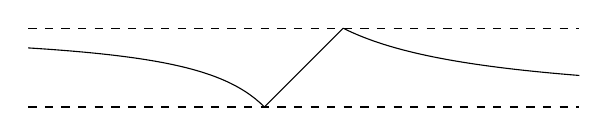
\begin{tikzpicture}
\draw(0,0)--(1,1);
\draw[dashed](-3,0)--(4,0);
\draw[dashed](-3,1)--(4,1);
\draw[domain=1:4,samples=50] plot (\x, {2/(\x+1)});
\draw[domain=-3:0,samples=50] plot (\x, {\x/(\x-1)});
\end{tikzpicture}
\end{figure}
\end{definition}

\begin{definition}[Kolmogorov classification of topological spaces]\index{Kolmogorov classification of topological spaces}
$X$ is a $T_0$ \textit{space} if for any two distinct points in $X$, at least one of them has a neighborhood which doesn't intersect the other piont, i.e. they are \textit{topologically distinguishable} \par
$X$ is a $T_1$ \textit{space} if for any two distinct points in $X$, each of them has a neighborhood which doesn't intersect the other point. $T_1$ $\Leftrightarrow$ points are closed \par
$X$ is a $T_2$ \textit{space} or \textit{Hausdorff space}\index{Hausdorff space} if any two distinct points have disjoint neighborhoods. Then the limit of $\{x_n\}$ is unique, denotes the limit $x=\lim x_n$ \par
$X$ is a $T_{2 {}^1{\mskip -5mu/\mskip -3mu}_2}$ \textit{space} or \textit{Urysohn space}\index{Urysohn space} if any two distinct points have disjoint closed neighborhoods \par
$X$ is a $T_3$ \textit{space} if $X$ is regular Hausdorff \par
$X$ is a $T_{3 {}^1{\mskip -5mu/\mskip -3mu}_2}$ \textit{space} if $X$ is completely regular Hausdorff \par
$X$ is a $T_4$ \textit{space} if $X$ is normal $T_1$ space $\Leftrightarrow$ normal Hausdorff \par
$X$ is a $T_5$ \textit{space} if $X$ is completely normal Hausdorff \par
$X$ is a $T_6$ \textit{space} if $X$ is perfectly normal $\Leftrightarrow$ perfectly normal Hausdorff
\end{definition}

\begin{definition}
$A\subseteq X$ is \textit{nowhere dense} if the interior of $\overline{A}$ is $\varnothing$
\end{definition}

\begin{definition}
$X$ is \textit{sequential compact} if every sequence has a convergent subsequence
\end{definition}

\begin{definition}
The \textit{box topology}\index{Box topology} on $\displaystyle\prod_{i\in I}X_i$ has base $\displaystyle\left\{\prod_{i\in I} U_i\middle|U_i\subseteq X_i\text{ open}\right\}$
\end{definition}

\begin{lemma}
$X$ is Hausdorff iff the diagonal $\{(x,x)|x\in X\}$ is closed
\end{lemma}

\begin{proof}

\end{proof}

\begin{definition}
$X\times I\xrightarrow{F}Y$ is a \textit{homotopy}\index{Homotopy} between $X\xrightarrow{f_0,f_1} Y$  if  $F(x,0)=f_0(x)$, $F(x,1)=f_1(x)$, write $f_t=F(\cdot,t)$. $X\xrightarrow{f} Y$ is a \textit{homotopy equivalence}\index{Homotopy equivalence} if there is $Y\xrightarrow{g} X$ such that $gf\simeq1_X$, $fg\simeq1_Y$
\end{definition}

\begin{definition}
$X\xrightarrow f Y$ is a \textit{topological embedding} if $f:X\to f(X)$ is a homeomorphism
\end{definition}

\begin{definition}
$K\subseteq X$ is \textit{compact}\index{Compact} if any open cover has a finite subcover. Equivalently, $K$ is disjoint from the intersection of a family of closed sets, then $K$ is disjoint from the intersection of finitely many of them \par
$X$ is \textit{locally compact}\index{Locally compact} if there is a compact neighborhood for each point \par
$Y\subseteq X$ is \textit{precompact}\index{Precompact} if $\overline Y$ is compact
\end{definition}

\begin{definition}
$A\subseteq X$ is \textit{dense}\index{Dense} if $\overline A=X$ \par
$X$ is \textit{separable}\index{Separable space} if $X$ has a countable dense subset
\end{definition}

\begin{definition}
$X_\alpha\subseteq X$, $\{X_\alpha\}$ is \textit{locally finite}\index{Locally finite} if for any $x\in X$, there is a neighborhood of $x$ intersecting only finitely many $X_\alpha$'s \par
$\mathcal U=\{U_\alpha\}$, $\mathcal V=\{V_\beta\}$ are covers of $X$, $\mathcal V$ is a \textit{refinement}\index{Refinement} of $\mathcal U$ if for any $V_\beta$, there exists $U_\alpha$ containing $V_\beta$ \par
$X$ is \textit{paracompact}\index{Paracompact} if every open cover has a locally finite open refinement
\end{definition}

\begin{lemma}
Closed subsets of compact space are closed \par
The image of a compact set is compact \par
Compact subsets of a Hausdorff space are closed
\end{lemma}

\begin{lemma}\label{X compact, Y Hausdorff, injective maps are embeddings}
$X$ is compact, $Y$ is Hausdorff, an injective map $X\xrightarrow fY$ is a topological embedding
\end{lemma}

\begin{proof}
$f:X\to f(X)$ is a continuous bijection. If $K\subseteq X$ is closed, $K$ is also compact since $X$ is compact, thus $f(K)$ is compact, $f(K)$ is also closed since $Y$ is Hausdorff
\end{proof}

\begin{definition}
$X$ is called \textit{connected}\index{Connected} if it can be written as the union of two open subsets \par
$X$ is called \textit{locally connected}\index{Locally connected} if for any $x\in X$, there is a local basis that are connected
\end{definition}

\begin{proposition}
Connected components are closed \par
Connectedness and local path connectedness implies path connectedness
\end{proposition}

\begin{remark}
Connected components may not be open
\end{remark}

\begin{definition}
$E\xrightarrow{p} B$ has \textit{lift extension property}\index{Lift extension property} for $(X,A)$ if for any $X\xrightarrow{f} B$, a lift $A\xrightarrow{\tilde f} E$ can be extended to $\tilde f:X\to E$
\begin{center}
\begin{tikzcd}
A \arrow[r, "\tilde f"] \arrow[d, hook]          & E \arrow[d, "p"] \\
X \arrow[ru, "\tilde f", dashed] \arrow[r, "f"'] & B               
\end{tikzcd}
\end{center}
$E\xrightarrow{p} B$ has \textit{homotopy lifting property}\index{Homotopy lifting property} for $(X,A)$ if it has lift extension property for $(X\times I,X\times\{0\}\cup A\times I)$
\end{definition}

\begin{proposition}
If $(X,A)$ satisfies homotopy extension property, and $A$ is contractible, then the quotient map $X\xrightarrow{q} X/A$ is a homotopy equivalence
\end{proposition}

\begin{proof}
Consider $X\times\{0\}\cup A\times I\to A\hookrightarrow X$, where $(x,0)\mapsto x$, $(a,1)\mapsto*$ can be extended to $f:X\times I\to X$, $f_0=1_X$, $f_1(A)=\{*\}$, thus $f_1$ induces $r:X/A\to X$, $f_1=rq$, $X\times I\xrightarrow{f} X\xrightarrow{q}X/A$ also induce $g:X/A\times I\to X/A$, where $qf_t=g_tq$, and $g_0=1_{X/A}$, $g_1=qr$ thus $qr\simeq 1_{X/A}$
\end{proof}

\begin{definition}
$U\subseteq X$ is open if $U\cap K$ is open for any compact subspace $K\subseteq X$ defines a topology. Equivalently, $F\subseteq X$ is closed if $F\cap K$ is closed for any compact subspace $K\subseteq X$. $X$ is \textit{compactly generated}\index{Compactly generated} if $X$ has this topology
\end{definition}

\begin{definition}
A map is \textit{proper}\index{Proper map} if the preimage of a compact set is compact \par
A map is \textit{discrete}\index{Discrete map} if the preimage of a discrete set is discrete
\end{definition}

\begin{definition}
$X$ has \textit{discrete topology}\index{Discrete topology} if $\tau=\mathcal{P}(X)$. $X$ has \textit{trivial topology}\index{Trivial topology} if $\tau=\{\varnothing,X\}$
\end{definition}

\begin{proposition}\label{Properties of discrete topology}
Suppose $X$ has discrete topology \par
\textit{(a) }Any map $f:Y\to X$ is continuous iff $f^{-1}(x)$ is open for all $x\in X$ \par
\textit{(b) }If continuous maps $f,g:X\to X$ are homotopic, then they are actually the same
\end{proposition}

\begin{proof} $\\$
\textit{(a) }For any subset $U\subseteq X$, $f^{-1}(U)=\bigcup_{x\in U}f^{-1}(x)$ is open\par
\textit{(b) }If $F:X\times I\to X$ is a homotopy, then the restriction on $\{x\}\times I$ is gives a continuous map $I\to X$, the image has to be connected, thus the restriction is a constant, thus $f(x)=F(x,0)=F(x,1)=g(x)$
\end{proof}

\begin{lemma}\label{Pasting lemma}
$F_i\subseteq X$ are closed, $\bigcup_iF_i=X$, $f|_{F_i}$ are continuous, then $f$ is continuous
\end{lemma}

\begin{lemma}\label{X compact + Y Hausdorff => f:X->Y quotient map}
If $X$ is compact, $Y$ is Hausdorff, a surjective continuous map $f:X\to Y$ is a quotient map
\end{lemma}

\begin{proof}
Let's use the universal property of quotient space, consider a continuous map $g:X\to Z$ such that $g$ maps fibers of $f$ to points, thus we have a map $\tilde g:Y\to Z$, $\tilde gf=g$, for any closed set $F$ in $Z$, so is $K=g^{-1}(F)=f^{-1}(\tilde g^{-1}(F))$, since $X$ is compact, so is $K$, hence $f(K)=\tilde g^{-1}(F)$ is compact, and since $Y$ is Hausdorff, $\tilde g^{-1}(F)$ is closed
\end{proof}

\begin{lemma}\label{X locally compact+Hausdorff, F closed iff F intersects K is compact for any K compact}
$X$ is locally compact, Hausdorff, $F\subseteq X$ is closed iff $F\cap K$ is compact for any compact subset $K\subseteq X$
\end{lemma}

\begin{proof}
$F$ closed $\Rightarrow F\cap K$ closed. Conversely, suppose $F\cap K$ is compact for any compact subsets $K\subseteq X$, for any $x\notin F$, there is a compact set $K$ containing an open neighborhood $U$ of $x$, $F\cap K$ is compact thus closed, hence $G=U-F\cap K$ is an open neighborhood of $x$ which is disjoint of $F$, hence $F$ is closed 
\end{proof}

\begin{lemma}
$X,Y$ are locally compact, Hausdorff, $p:X\rightarrow Y$ is continuous, proper, then $p$ is closed
\end{lemma}

\begin{proof}
Suppose $F\subseteq X$ is closed, since $p\left(F\cap p^{-1}(K)\right) = p(F)\cap K$, by Lemma \ref{X locally compact+Hausdorff, F closed iff F intersects K is compact for any K compact}, we can take any $K\subseteq Y$ compact, hence $F$ is closed
\end{proof}

\begin{definition}
$X$ is noncompact, the \textit{Alexandorff extension}\index{Alexandorff extension} of $X$ is $X^*=X\cup\{\infty\}$ with open sets $\varnothing, X^*$, open sets in $X$ and complements of closed compact sets of $X$ \par
$X \hookrightarrow X^*$ is an open topological embedding \par
If $X$ is also locally compact Hausdorff, $X^*$ is the \textit{one point compactification}\index{One point compactification} of $X$ which is Hausdorff
\end{definition}

\begin{lemma}\label{X,Y locally compact Hausdorff, f:X->Y proper, f send discrete sets to discrete sets}
$X,Y$ are locally compact Hausdorff, $X\xrightarrow{f}Y$ is proper, then $f$ sends discrete sets to discrete sets
\end{lemma}

\begin{proof}
Suppose $A\subseteq X$ is discrete, $x_0\in A$, $y_0=f(x_0)\in Y$, $K$ is a compact neighborhood of $y_0$, then $f^{-1}(K)$ is a compact neighborhood of $x_0$, thus $f^{-1}(K)\cap A$ is finite, so is $K\cap f(A)$, since $Y$ is Hausdorff, there is a neighborhood $U$ of $y_0$ such that $U\cap f(A)=y_0$
\end{proof}

\begin{lemma}
$X,Y$ are locally compact, $X\xrightarrow{p}Y$ is proper and discrete, then $p^{-1}(y)$ is finite, and for any neighborhood $V$ of $p^{-1}(y)$, there is a neighborhood $U$ of $y$ such that $p^{-1}(U)\subseteq V$
\end{lemma}

\begin{lemma}
$X,Y$ are locally compact Hausdorff, $X\xrightarrow{p}Y$ is a proper local homeomorphism, then $p$ is a finite sheeted covering
\end{lemma}

\begin{definition}
The \textit{compact-open topology}\index{Compact-open topology} on $Y^X$ is given by a subbase $V(K,U):=\left\{f\in Y^X\middle|f(K)\subseteq U\right\}$, with $K\subseteq X$ compact and $U\subseteq Y$ open \par
A \textit{normal family}\index{Normal family} $\{f_i\}$ is a precompact subset of $Y^X$
\end{definition}

\begin{lemma}
$\{f_n\}$ converges pointwise on $X$ iff $\{f_n\}$ converges in $Y^X$ with the product topology $\displaystyle\prod_{x\in X}Y$. Hence we call the product topology the \textit{topology of pointwise convergence}\index{Topology of pointwise convergence}
\end{lemma}

\begin{proof}
If $f_n$ converges pointwise on $X$ to $f$, then for any neighborhood $V_i$ of $f(x_i)$, $i=1,\cdots,k$, $V_k$ contains all but finitely many $f_n(x_i)$, thus for $n$ big enough, $\displaystyle f_n\in V_1\cap\cdots\cap V_k\cap\prod_{x\neq x_0}Y$, i.e. $\{f_n\}$ converges to $f$ in $Y^X$
\end{proof}

\begin{theorem}
$X$ is compact, $Y$ is a complete metric space, then the topology induced by metric $\displaystyle d(f,g)=\sup_{x\in X}d(f(x),g(x))$ is the same as the compact-open topology on $Y^X$
\end{theorem}

\begin{theorem}
$Y^*\cong Y$
\end{theorem}

\begin{theorem}
The composition $Z^Y\times Y^X\to Z^X,(g,f)\mapsto g\circ f$ is continuous, in particular, if $X=*$, then this becomes the evaluation map $\mathrm{eval}:Z^Y\times Y,(f,y)\mapsto f(y)$
\end{theorem}

\begin{theorem}
$Z^{X\times Y}\cong \left(Z^{Y}\right)^X$
\end{theorem}

\begin{definition}
A topological space $X$ is reducible if $X=X_1\cup X_2$, $X_1,X_2$ are proper nonempty closed subsets, $X_1\nsubseteq X_2$, $X_2\nsubseteq X_1$, $X$ is \textit{irreducible}\index{Irreducible topological spaces} if not reducible
\end{definition}

\begin{definition}
A topological space $X$ is \textit{Noetherian}\index{Noetherian topological space} if $X\supsetneqq X_1\supsetneqq X_2\supsetneqq\cdots$ terminates, $\displaystyle\dim V=\sup_d(X_0\supsetneqq X_1\supsetneqq\cdots\supsetneqq X_d)$, $V_i$'s are closed and irreducible
\end{definition}

\begin{theorem}[Tychonoff's theorem]\label{Tychonoff's theorem}
$\{K_i\}_{i\in I}$ are compact, so is $\displaystyle\prod_{i\in I}K_i$
\end{theorem}

\begin{proposition}
Connected sets of $\mathbb R$ are intervals $(a,b)$, $[a,b)$, $(a,b]$ or $[a,b]$
\end{proposition}

\begin{theorem}[Jordan curve theorem]\label{Jordan curve theorem}\index{Jordan curve theorem}
$S^n\xrightarrow{i}\mathbb R^{n+1}$ is injective thus an open embedding by Lemma \ref{X compact, Y Hausdorff, injective maps are embeddings}, denote $X=i(S^n)$, then $Y=\mathbb R^{n+1}\setminus X$ consists of exactly two connected components, the interior $U$ which is bounded, and the exterior $V$ which is not. When $n=1$, $U$ and $V$ are homeomorphic to $D$ and $\mathbb R^2\setminus D$
\end{theorem}

\begin{definition}
$W\subseteq X$ is a \textit{locally closed set}\index{Locally closed set} if for any point $p\in W$, there is an open neighborhood $U\ni p$ such that $U\cap W$ is closed in $U$. Equivalently, $W$ is the intersection of an open subset and a closed subset, or equivalently, $W$ is relatively open in $\overline W$. A \textit{constructible set}\index{Constructible set} is a finite union of locally closed sets
\end{definition}

\begin{theorem}[Lefschetz fixed point theorem]\index{Lefschetz fixed point theorem}\label{Lefschetz fixed point theorem}
$X$ is a compact triangulable space of dimension $n$, the \textit{Lefschetz number}\index{Lefschetz number} of $f$ is $\displaystyle\sum_{k=0}^n\tr(f_*|_{H_k(X;\mathbb Q)})$. If the Lefschetz number of $f$ is nonzero, then $f$ has fixed points. The converse is not true, i.e. even if the Lefschetz number is zero, then could be fixed points \par
If $f=\id_X$, then the Lefschetz number is the Euler characteristic $\chi$
\end{theorem}

\begin{definition}
The \textit{join}\index{Join} of $X,Y$ is
\[X*Y=\frac{X\times Y\times I}{(x,y_1,0)\sim(x,y_2,0),(x_1,y,1)\sim(x_2,y,1)}\]
We can also interpret it as all possible paths from $X$ to $Y$. In general, $\underset{i}{*}X_i$ can be thought of as finite sum $\displaystyle\sum_it_ix_i$, $t_i\in I$, $x_i\in X_i$
\end{definition}

\begin{definition}
$X$ is \textit{Noetherian} if every descending chain of subspaces is finite
\end{definition}

\begin{proposition}
\begin{enumerate}
\item Subspaces of Noetherian spaces are Noetherian
\item $X$ is Noetherian iff $X$ is locally Noetherian and compact
\end{enumerate}
\end{proposition}

\begin{proof}
\begin{enumerate}
\item A descending chain of a subspace is also a descending chain
\item 
\end{enumerate}
\end{proof}

\begin{definition}
A covering space is a fiber bundle with discrete fibers
\end{definition}

\begin{proposition}\label{Unique lifting iff fundamental group is a subgroup}
$Z\xrightarrow pX$ is a covering, $f(y_0)=p(z_0)$. $f$ lifts $\tilde f: Y\to Z$ with $f(y_0)=z_0$ iff $f_*\pi_1(Y,y_0)\leq p_*\pi_1(Z,z_0)$
\begin{center}
\begin{tikzcd}
                                                  & Z \arrow[d, "p"] \\
Y \arrow[r, "f"'] \arrow[ru, "\exists_1\tilde f"] & X               
\end{tikzcd}
\end{center}
\end{proposition}

\begin{proposition}
Covering $Y\xrightarrow p X$ is regular if $\Aut(Y/X)$ is a normal subgroup of $\pi_1(X,x_0)$
\end{proposition}

\begin{proof}
Assume $p(y_1)=p(y_2)=x_0$, by Proposition \ref{Unique lifting iff fundamental group is a subgroup}, $p_*\pi_1(Y,y_1)=p_*\pi_1(Y,y_2)$ are conjugate, hence normal
\end{proof}

\begin{definition}
$A\xrightarrow iX$ is inclusion. A \textbf{deformation}\index{Deformation} of $A$ into $B\subseteq X$ in $X$ is a homotopy $A\xrightarrow{f_t} X$ such that $f_0=i$ and $f_1(A)\subseteq B$, onto if equality holds. $X\xrightarrow rA$ is a \textbf{retraction}\index{Retraction} if $ri=1_A$. $r$ is a \textbf{weak retraction}\index{Weak retraction} if inclusion $A\xrightarrow iX$ has a left homotopy inverse, i.e. $ri\simeq1_A$. A \textbf{deformation retraction}\index{Deformation retraction} is a deformation $X\xrightarrow{f_t} X$ such that $f_1=ri$ for some retraction $X\xrightarrow rA$. Deformation retraction $f_t$ is \textbf{strong}\index{Strong deformation retraction} if $f_t|_A=1_A$ \par
$X$ is \textbf{contractible}\index{Contractible} if $X$ deformation retracts onto a point \par
$(X,A)$ is a \textbf{good pair}\index{Good pair of topological spaces} if $A$ is a strong neighborhood deformation retract of $X$
\end{definition}

\begin{lemma}\label{Some rudimentary lemma about retract and deformation}
$A\xrightarrow iX$ is inclusion 
\begin{enumerate}[leftmargin=*]
\item $X$ is deformable into $A$ iff $i$ is a \textbf{weak section}, namely $i$ has a right homotopy inverse, i.e. $ir\simeq 1_X$ 
\item $i$ is a homotopy equivalence iff $A$ is a weak retract of $X$ and $X$ is deformable into $A$ 
\item If $X$ is deformable into a retract $A$, then $A$ is a deformation retract of $X$
\item If $(X,A)$ is cofibered, then $A$ is a weak retract of $X$ iff $A$ is a retract of $X$
\end{enumerate}
\end{lemma}

\begin{proof}
\begin{enumerate}[leftmargin=*]
\item If $X\times I\xrightarrow HX$ is a homotopy from $1_X$ to $ir$, then $H$ is a deformation of $X$ into $A$ since $H_0=1_X$, $H_1(X)\subseteq A$. If $H$ is a deformation of $X$ into $A$, since $H_1(X)\subseteq A$, define $X\xrightarrow rA$ such that $ir=H_1$, then $r$ is a right homotopy inverse of $i$
\item $i$ is a homotopy equivalence $\Leftrightarrow$ there exists $X\xrightarrow rA$ such that $ri\simeq 1_A$, $1_X\overset{H}{\simeq}ir$ $\Leftrightarrow$ $r$ is a weak retract, $H$ is a deformation of $X$ into $A$
\item $X\xrightarrow rA$ is a retraction, $X\times I\xrightarrow HX$ is a deformation of $X$, then $1_X\simeq ir'$ for some $X\xrightarrow {r'}A$, hence $r\simeq rir'=r'$ $\Rightarrow$ $1_X\simeq ir\simeq ir$ giving a deformation retract 
\item $A\times I\xrightarrow HA$ is a homotopy from $ri$ to $1_A$, since $r(a)=H_0(a)$ and $(X,A)$ is cofibered, we have $X\times I\xrightarrow FA$, then $F_0=r$, $F_1i=1_A$, i.e. $r$ is homotopic to retraction $F_1$
\end{enumerate}
\end{proof}

\begin{definition}
$\mathcal C$ is a class of topological spaces closed under homeomorphism and closed subsets. $X$ is an \textbf{absolute retract}\index{Absolute retract} for $\mathcal C$ if for $Y\in \mathcal C$, embedding $X\hookrightarrow Y$ is closed $\Rightarrow$ $X$ is a retract of $Y$. $X$ is an \textbf{absolute neighborhood retract}\index{Absolute neighborhood retract} for $\mathcal C$ if for $Y\in \mathcal C$, embedding $X\hookrightarrow Y$ is closed $\Rightarrow$ $X$ is a neighborhood retract of $Y$
\end{definition}

\end{document}